\question 一个进程是
\par\twoch{由处理器执行的一个程序}{一个独立的程序和数据集}{\textcolor{red}{PCB结构与程序和数据的结合}}{一个独立的程序}
\begin{solution}进程是由PCB、程序段和数据段构成的,进程的主要信息都保存在PCB中。A选项没有包含数据段,不是完整的进程;B选项描述的是静态的程序和数据集,不符合进程的动态性特点;D选项的描述明显错误。
★PCB是操作系统感知进程存在的唯一依据。
\end{solution}
\question (北京理工大学,2001年)在进程的生命周期内,进程与其执行的程序个数之间是(
)关系
\par\twoch{一对一}{一对多}{多对一}{\textcolor{red}{多对多}}
\begin{solution}可能存在一个进程执行一个程序的情况,即为一对一关系。
可能存在一个进程执行多个的程序的情况,即为一对多关系。
可能存在一个程序被多个进程执行的情况,即为多对一关系。
因此本题最合适的答案是D。
\end{solution}
\question (燕山大学,2006年)下面哪个特征是并发程序执行的特点
\par\twoch{\textcolor{red}{程序执行的间断性}}{相互通信的可能性}{产生死锁的可能性}{资源分配的动态性}
\begin{solution}与程序顺序执行对比,程序并发执行时的特征有以下几个方面。 
间断性:并发程序具有``执行---暂停---执行''这种间断性的活动规律。 
失去封闭性:多个程序共享系统中的各种资源,因而这些资源的状态将由多个程序来改变,致使程序的运行已失去了封闭性。

不可再现性:由于失去了封闭性,程序的计算结果与并发程序的执行速度有关,从而使程序失去了可再现性。
\end{solution}
\question 关于优先级大小的论述中,正确的是
\par\fourch{计算型作业的优先级,应高于I/O型作业的优先级}{用户进程的优先级,应高于系统进程的优先级}{在动态优先级中,随着作业等待时间的增加,其优先级将随之下降}{\textcolor{red}{在动态优先级中,随着进程执行时间的增加,其优先级将随之下降}}
\begin{solution}优先级应当与进程或作业的紧急程度或者要完成的功能有关系,与作业类型并没有绝对的关系,也与用户级和系统级没有必然的关系。
动态优先级中,随着作业等待时间的增加,优先权会随之增加,随着进程执行时间的增加,优先权随之降低。这样才能保证作业在有限等待的时间内得到执行,否则等待时间越长,优先级越低,一直得不到调度而饿死。
\end{solution}
\question 一个多道批处理系统中仅有P1和P2两个作业,P2比P1晚5ms到达。它们的计算和I/O操作顺序如下:
P1:计算60ms,I/O 80ms,计算20ms P2:计算120ms,I/O 40ms,计算40ms
若不考虑调度和切换时间,则完成两个作业需要的时间最少是( )
\par\twoch{240ms}{\textcolor{red}{260ms}}{340ms}{360ms}
\begin{solution}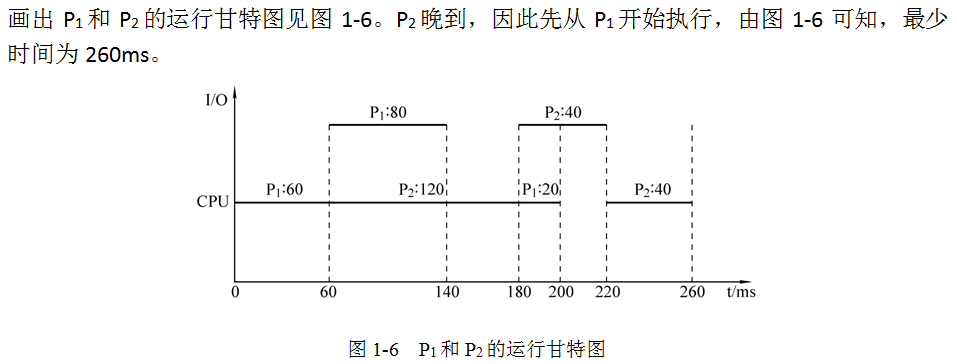
\includegraphics[width=3.46875in,height=1.32292in]{computerassets/9B057B841FA35D592A38935D909C62F2.png}
\end{solution}
